\section{Introduction}
\begin{sectionplan}
     \begin{itemize}
          \item  General introduction extoling how prevalant compilers are
                 and how everyone and their mother is using them in some form
                 or another.

          \item Justify further research into compilers based on their use
                in software development and other fields.

          \item Talk about research into parallel compilers at a highlevel,
                ie the current state of research, when research has been done,
                parallel compilers historically of low importance.

          \item Link to next section that describes how compilers work at a
                high level
     \end{itemize}
\end{sectionplan}

Compilers are an important part of the interface between a programmer and the
machine for which he is developing software. The modern software ecosystem
could not exist without the frequent and extensive use of compilers in the
software development process. It is of no surprise that the study of compilers
and programming languages has been an important field of research in computer
science for many decades. Any improvements in compiler technology can have wide
and long lasting affects on software development speed and software quality
which makes compiler research strongly worthwhile \citep{hall_compiler_2009}

Compiler research can generalize to other areas outside of software development.
Applications of techniques traditionally associated with compilers can be
found in network packet parsing \citep{wang_hyperscan_2019, roesch_snort_1999}
and huffman decoding \citep{howard_parallel_1996}. These areas, among others,
can benefit from research directed at improving compiler technology due to a
significant overlap in the underlying theory
\citep{mytkowicz_data-parallel_2014}. It is evident that futher development in
compiler theory can be justified not only by its direct benefit to software
development but also its affect on tangential fields of research.

The focus of my FYP is to study a subset of compiler research regarding parallel
compiler implementations. Research into this niche has been historically
of low priority. Traditional compiler architecture in the 70’s was focused
on minimising memory use and optimising for single threaded performance
(\textbf{citation needed}). This was at a time when computers didn’t even
have enough ram to store all the data necessary for compiling a large amounts
of source code. Times have since changed. The memory available in a computer
is much more abundant than before and single threaded processor speed is not
improving at the same rate as it once did (\textbf{citation needed}). In fact,
were seeing commodity processors contain many cores capable of running dozens of
threads in parallel. I believe this is sufficient cause to consider alternative
architectures that better utilise this environment.

\begin{roughwork}

     Language design decisions of that era were made to address this problem.
     For example, in C, programmers are forced to declare functions before
     they are called. This was originally done to allow the compiler to
     fully compile each function independantly, without needing to keep all
     the other functions in memory and avoiding a costly second pass over
     code (\textbf{citation needed}). 

\end{roughwork}


\subsection{Sequential Compilation}
\begin{sectionplan}
     Short explanation of compiler technology and the structure of a compiler.
     Explain the compilation process and the use cases for compilation.
\end{sectionplan}

\begin{figure}[t]
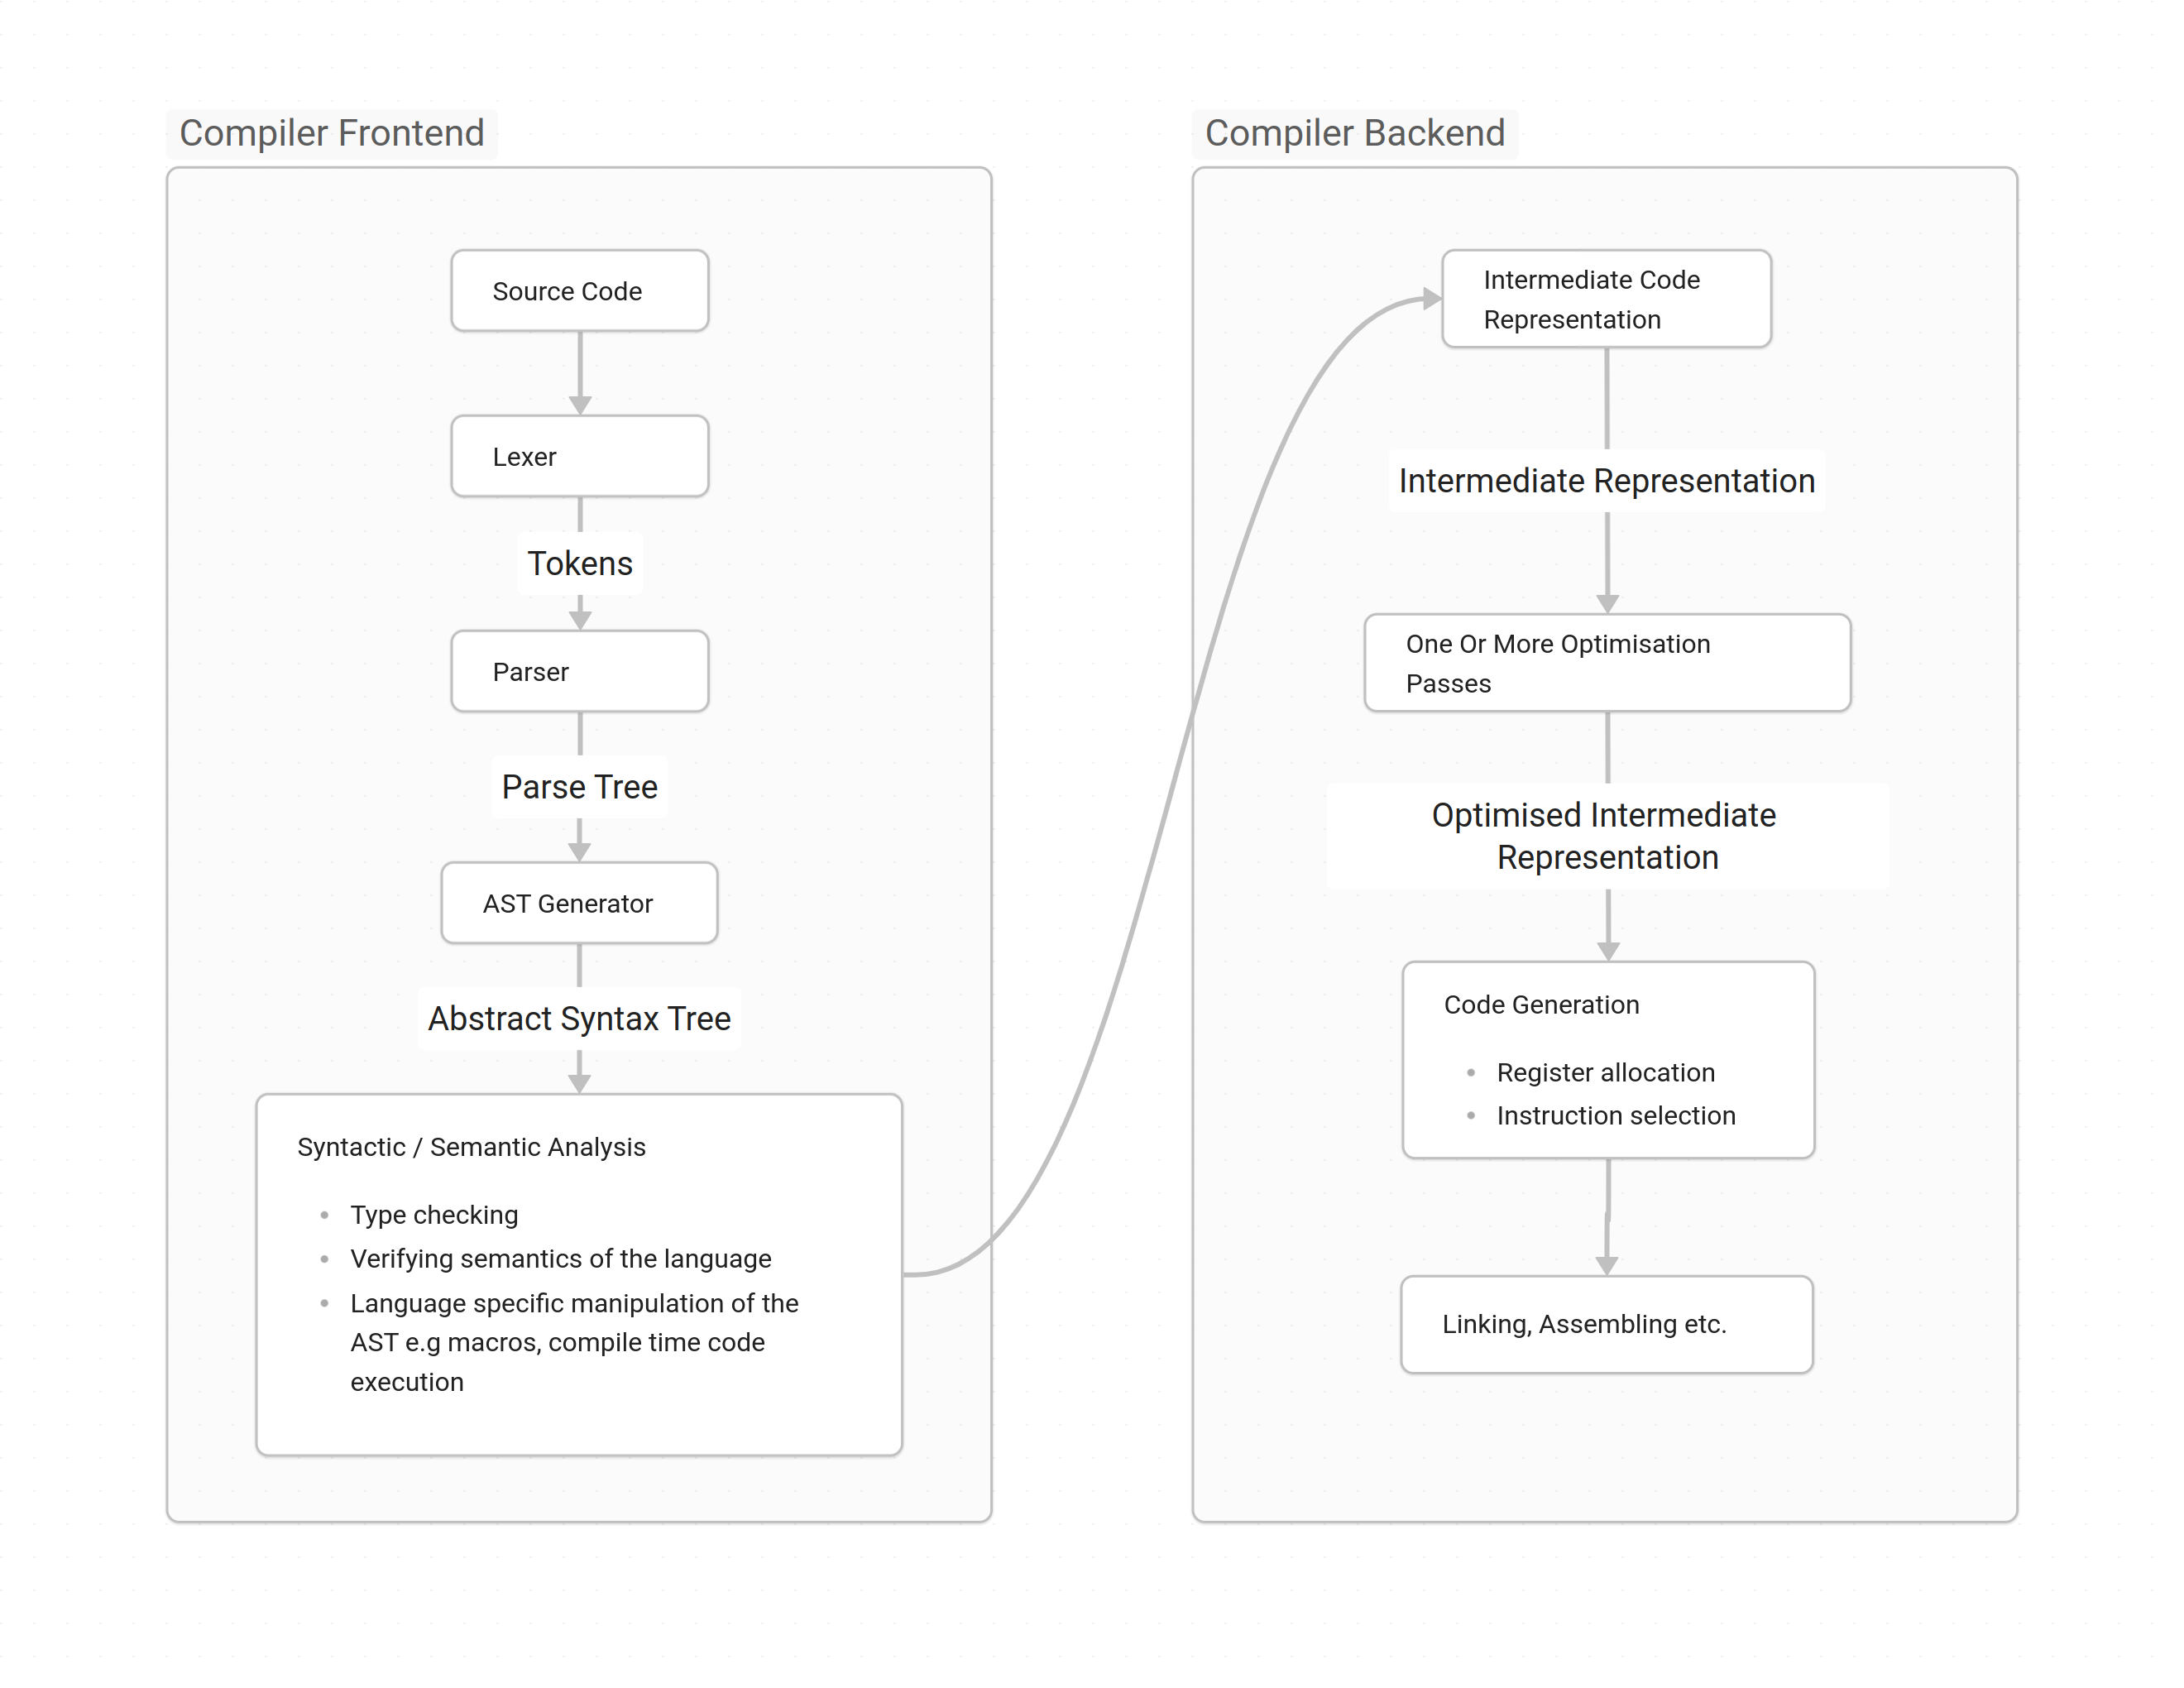
\includegraphics[width=\linewidth]{images/generic_compiler.png}
\centering
\caption{Diagram of compilation phases in a generic compiler}
\label{fig:compiler}
\end{figure}

The function of a compiler is to transform source code from one language into
another. During this process, a compiler will usually lose information in the
source code that is useful to the programmer but useless to the machine that
will execute the program. Inside a compiler, the source code passes through
several algorithms that transform the code in various ways. These different
compilation stages are visualised in figure \ref{fig:compiler}.

Compilers work in a sequential way that resemebles a pipeline. The lexer splits
up the source code into words called tokens. The parser then takes those tokens
and assigns structure to them by arraging them as a graph. This structure makes
them easier to meaningfully navigate. It addtionally lets the tokens better describe
what they mean, beyond what can be understood from a simple list of words. This
graph of tokens is then analysed during the semantic analysis phase, doing
things like looking for unsused variables. The parts of the compiler up to this
point are colloquially called the frontend of the compiler.


\subsection{Parallel Compiliation}
\begin{sectionplan}
    \begin{itemize}
	\item What is meant by parallelism in a compiler implementation as  compared to
          a compiler generating code that works in parallel.

	\item Justify looking at alternative forms of parallelism besides the status quo
          method of compiling source files in parallel and linking them together
          in the end.

		\begin{itemize}
         	\item Finer grained parallelism is better suited for running code on 				
				  massively parallel hardware like GPU's.

         	\item More parts of a program can be compiled in parallel which makes
				  better use of a computers parallel processing facilities. Mention 
				  ahmdals law.

         	\item Reduced bottle neck when compiling very large files (since
				  individual files are split up and compiled in parallel).

			\item Significant speedups in other fields where only one stage of is 
				  needed like lexing and parsing very large amounts of structured 
				  data. Mention PAPAGENO parser with relation to simdjson.
		\end{itemize}

    \end{itemize}
\end{sectionplan}

The stages of a compiler that are reponsible for taking a file from
source code to code generation are often implemented with little to no
parallelisation(\textbf{citation needed}). An example of going from source code
to machine code is the process of compiling a C file into an object file. As
can be seen from figure \ref{fig:compiler}, this envelopes a significant portion
of the compiler. Many existing compilers can operate in parallel by compiling
several source code files at the same time. In this work I am looking at methods
employing finer-grained parallelism where various stages of a compiler can be
executed in parallel. These are methods described in more detail in Section
\ref{compiler_parallel_methods}.


\subsubsection{Parallel As Compared To Sequential}
\begin{sectionplan}
     Reasons why parallel compilation is good / better.

     \begin{itemize}
          \item More cores used during compilation increase compiler performance
                and better overall system usage

          \item Hardware investments in the industry involve specialisation
                and increasing reliance on performance gained from parallel
                architectures. Existing compilers cannot benefit from this.

          \item Choosing a language syntax as a language designer based on how
                well it can be processed in parallel in the future is necessary
                early on. Making those choices is difficult due to a lack of
                research.
     \end{itemize}
\end{sectionplan}

Using multiple CPU cores during compilation can speed up compilation time.
Researchers in 2009 created an optimised lexer for a machine that had a large
number of cores that could run code in parallel
\citep{scarpazza_high-performance_2009}. It had eight cpu cores where each core
could run eight threads in parallel for a total of 64 parallel threads.  This
shows how using parallel processing to speed up compilation tasks is not a new
idea. Subsequent research into parallel lexing from 2014 achieved a 14 times
speed up for lexing HTML on a 16 core system
\citep{mytkowicz_data-parallel_2014}. Substantial performance gains can clearly
be achieved through parallelisation.

There have been increasingly larger investments in the hardware industry for
specialised hardware beyond the typical CPU. Examples include things like smart
nics that offload network packet parsing from the CPU or DPU’s that provide
more facilities for networking and input / output related tasks than a typical
CPU. A recent article from October 2023 shows how AMD’s software stack for
general purpose computing on graphics cards known as rocm is now among their top
priorities \citep{ward-foxton_rocm_2023}. As time goes on, we are likely to see increasingly specialised and
heterogenous hardware (\textbf{citation needed}). Traditional compiler architecture is not well suited to
this type of environment.

For many programming languages, once a syntax goes into general use, it becomes
nearly impossible to revert or change it in a way that breaks existing programs.
This leads to programming languages becoming complicated and hard to define as
new features are added. For example, langauges like c++ are extremely hard to
compile in any way, let alone a parallel way. Research into and the development
of parallel compilers can aid future developers when they are choosing their
syntax or what features they want to implement without making their language
hard to compile in parallel (\textbf{citation needed}). It is currently
rather difficult to design a language that can easily be compiled in parallel
due to a lack of research and prior work compared to sequential approaches
(\textbf{citation needed}).

\subsection{Objectives of My Work}

The goal of my project is to research ways of the compilation stages in
a compiler frontend by using parallel processing methods, aswell as an
implementation of those stages if time allows.

\subsection{Outline of Subsequent Sections}

Section \ref{litreview} describes literature I have reviewed. In Section
\ref{design} I discuss the various approaches mentioned in the literature
review and their pros and cons. I elaborate the issues with designing a
parallel compiler aswell as the design of my compiler implementation. In Section
\ref{implementation} I explain the details of my implementation, explaining
things like external dependancies and code structure. Finally, I test and
evaluate the performance of my implementation in section \ref{evalandtesting},
followed by the conclusion in section \ref{conclusion}.